\section{Fahrstraßenlogik}\label{text:Entwicklung-des-Stellwerks:Fahrstrassenlogik}

Für die Bildung der Fahrstraßen wurde sich für das topologische Prinzip entschieden, da es die größte Flexibilität liefert. Die informationstechnische Abbildung eines topologischen Gleisplans ist ein Graph. Die beiden gängigsten Methoden, einen Graphen programmatisch darzustellen, sind eine Adjazenzliste und eine verkette Liste, wobei in diesem Projekt eine Adjazenzliste verwendet wurde.

In \autoref{abb:Entwicklung-des-Stellwerks:Fahrstrassenlogik:Bahnhof-Graph} ist der Graph des in \autoref{abb:Entwicklung-des-Stellwerks:Bahnhof-Gleisplan} dargestellten Gleisplans zu sehen.

\begin{figure}[H]
    \centering
    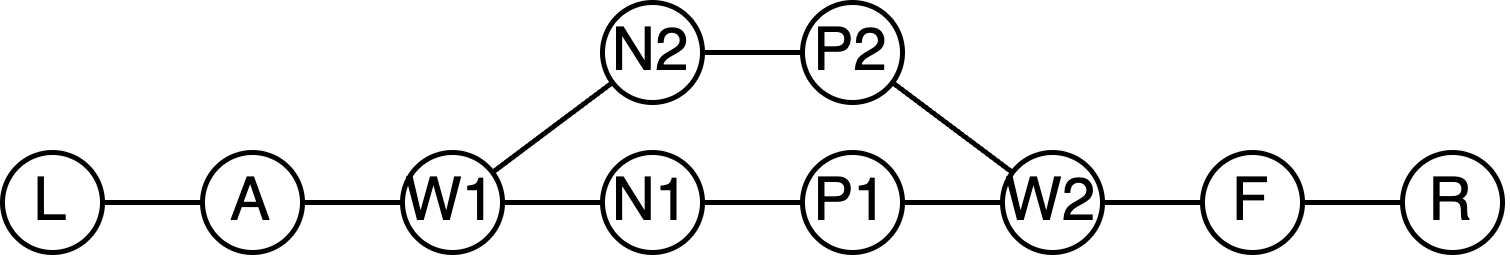
\includegraphics[width=\textwidth]{Assets/Images/5-Entwicklung-des-Stellwerks/Bahnhof-Graph.png}
    \caption{Gleisplan des Bahnhofs als Graph}\label{abb:Entwicklung-des-Stellwerks:Fahrstrassenlogik:Bahnhof-Graph}
\end{figure}

Dieser Graph kann dann wie in \autoref{abb:Entwicklung-des-Stellwerks:Fahrstrassenlogik:Bahnhof-Adjazenzliste} in einer Adjazenzliste dargestellt werden:

\begin{figure}[H]
    \centering
    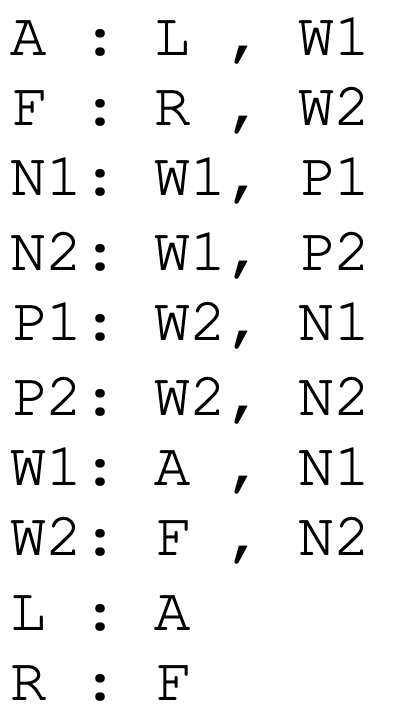
\includegraphics[width=.2\textwidth]{Assets/Images/5-Entwicklung-des-Stellwerks/Bahnhof-Adjazenzliste.png}
    \caption{Gleisplan des Bahnhofs als Adjazenzliste}\label{abb:Entwicklung-des-Stellwerks:Fahrstrassenlogik:Bahnhof-Adjazenzliste}
\end{figure}

Diese Liste, die streng genommen ein assoziatives Array ist, kann in einer einfachen Datenstruktur gespeichert werden. Zur Bildung einer Fahrstraße werden mithilfe der Depth-First-Search alle möglichen Pfade des Graphen gefunden. Anschließend wird der beste Pfad ausgewählt, der dann als Fahrstraße gestellt wird. Im hier verwendeten Beispiel würden für die Fahrstraße \(A \rightarrow P1\) die Pfade

\[A \rightarrow W1 \rightarrow N1 \rightarrow P1\] und
\[A \rightarrow W1 \rightarrow N2 \rightarrow P2 \rightarrow W2 \rightarrow P1\]

gefunden werden. Letzterer ergibt zwar mathematisch Sinn, kann aber aufgrund der Weiche nicht befahren werden. Daher ist eine Filterung notwendig, die schon in der Suche an einer Weiche entscheidet, ob ein Pfad logisch ist oder nicht. In diesem Fall würde die Fahrstraße folgendermaßen aussehen:

\[A: Fahrt!\]
\[W1: rechts\]
\[N1: Halt!\]
\[P1: Halt!\]

Die Software prüft nun, ob die benötigten Fahrwegelemente frei sind und stellt sie in die entsprechenden Positionen. Ist die Fahrstraße nicht möglich, weil eine Weiche zum Beispiel Teil einer anderen Fahrstraße ist, wird die Fahrstraße nicht gestellt und ein Fehler ausgegeben. Zum Stellen von Signalen und Weichen werden die Befehle an die jeweiligen Decoder geschickt.
